% Workshop: KDAI / IWT — External presentation on DDB research arc
% Presenter: Mary Ann Tan, FIZ-KDAI
% Audience: External researchers, potential collaborators
% TODO: Fill in event name and date before use
\documentclass[xcolor,aspectratio=169,compress]{beamer}
\usetheme{Boadilla}
\definecolor{maincolor}{rgb}{.38,.06,.80}
\usecolortheme[named=maincolor]{structure}
\usepackage{sansmath}
\usepackage{svg}
\usepackage{tikzsymbols}
\usepackage{tikz}
\usetikzlibrary{arrows.meta,positioning,fit,backgrounds}
\usepackage{array}
\usepackage{booktabs}
\usepackage{colortbl}
\usepackage{pifont}
\usepackage{fontawesome5}

\newcommand{\cmark}{\textcolor{green!60!black}{\ding{51}}}
\newcommand{\xmark}{\textcolor{red}{\ding{55}}}

\makeatother
\setbeamertemplate{footline}
{
  \leavevmode%
  \hbox{%
  \begin{beamercolorbox}[wd=.30\paperwidth,ht=2.25ex,dp=1ex,center]{author in head/foot}%
    \usebeamerfont{author in head/foot}\insertshortauthor{}
    (\insertshortdate)
  \end{beamercolorbox}%
  \begin{beamercolorbox}[wd=.55\paperwidth,ht=2.25ex,dp=1ex,center]{title in head/foot}%
    \usebeamerfont{title in head/foot}\insertshorttitle\hspace*{3em}
  \end{beamercolorbox}%
  \begin{beamercolorbox}[wd=.15\paperwidth,ht=2.25ex,dp=1ex,right]{date in head/foot}%
   \insertframenumber{} / \inserttotalframenumber\hspace*{1ex}
  \end{beamercolorbox}}%
  \vskip0pt%
}
\makeatletter

\setbeamertemplate{headline}[default]
\setbeamertemplate{navigation symbols}{}
\mode<beamer>{\setbeamertemplate{blocks}[rounded][shadow=false]}
\setbeamercovered{transparent}
\useoutertheme[subsection=false]{miniframes}

\title[DDB Research Arc]{From Babel to Memory Atlas:\\
  Semantic Enrichment of the German Digital Library}

\author[M.A.\ Tan]{
  \includesvg[width=.35\textwidth]{beamer-bodilla-template/Logo/FIZ_Logo_en.svg}\\[.8cm]
  Mary Ann Tan}

\institute[FIZ-KDAI]{FIZ Karlsruhe -- Leibniz Institute for Information Infrastructure, KDAI}

% TODO: replace with actual event name and date
\date[IWT, 2026]{[Event Name], 2026}

\logo{\includesvg[width=.2\textwidth]{beamer-bodilla-template/Logo/FIZ_Logo_en.svg}\vspace{215pt}}

% % % % % %
\begin{document}

% ===== TITLE SLIDE =====
\frame[plain]{\titlepage}

% ===== OUTLINE =====
\begin{frame}{Overview}
  \begin{columns}
    \begin{column}{.52\textwidth}
      \textbf{Three connected research threads:}
      \smallskip
      \begin{enumerate}\setlength{\itemsep}{6pt}
        \item \textbf{The problem} --- 65M DDB objects,
              structurally uniform but semantically opaque
        \item \textbf{MOCHO} --- mid-level ontology for
              cross-domain alignment (babel-ddb)
        \item \textbf{GeMeA} --- knowledge graph browser
              for the DDB (ISWC 2026 Resource Track)
        \item \textbf{GND Work Linking} --- NER pipeline
              for 4.5M German bibliographic title strings
      \end{enumerate}
    \end{column}
    \begin{column}{.45\textwidth}
      \begin{block}{Research arc}
        \begin{center}
          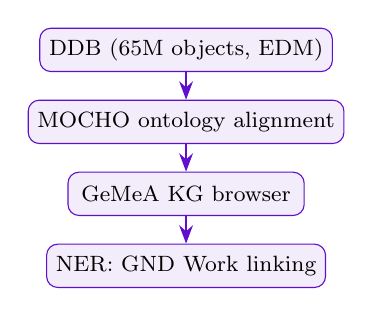
\begin{tikzpicture}[
            box/.style={draw=maincolor, fill=maincolor!8, rounded corners,
                        minimum width=3.0cm, minimum height=0.55cm,
                        font=\footnotesize, align=center},
            arr/.style={-Stealth, maincolor, thick}
          ]
            \node[box] (ddb)   {DDB (65M objects, EDM)};
            \node[box] (mocho) [below=0.35cm of ddb]  {MOCHO ontology alignment};
            \node[box] (gemea) [below=0.35cm of mocho] {GeMeA KG browser};
            \node[box] (ner)   [below=0.35cm of gemea] {NER: GND Work linking};
            \draw[arr] (ddb)   -- (mocho);
            \draw[arr] (mocho) -- (gemea);
            \draw[arr] (gemea) -- (ner);
          \end{tikzpicture}
        \end{center}
      \end{block}
    \end{column}
  \end{columns}
\end{frame}

% ===== 1. THE BABEL PROBLEM =====
\section{Problem}

\begin{frame}{The German Digital Library as a Library of Babel}
  \begin{columns}
    \begin{column}{.52\textwidth}
      \textbf{The DDB aggregates 65M cultural heritage objects} from archives,
      libraries, museums, and audiovisual archives into a structurally uniform
      container --- the Europeana Data Model (EDM).
      \medskip

      \begin{itemize}\setlength{\itemsep}{4pt}
        \item All objects become \texttt{edm:ProvidedCHO} --- one class regardless of type
        \item \texttt{dc:contributor} conflates author, editor, illustrator, director
        \item \texttt{dc:type} uncontrolled: thousands of free-text strings for
              the same concept
        \item Cross-domain discovery fails: ``Goethe's \textit{Faust}'' returns a book
              edition, a playbill, a film still, and an opera recording ---
              no connection between them
      \end{itemize}
    \end{column}
    \begin{column}{.45\textwidth}
      \begin{tabular}{ll}
        \toprule
        Sector & Objects \\
        \midrule
        Library     & $\sim$18.6M \\
        Media Library & $\sim$1.8M \\
        Museum      & $\sim$2.0M \\
        Archive     & $\sim$3.6M \\
        Research    & $\sim$1.2M \\
        Others      & $\sim$0.1M \\
        \midrule
        \textbf{Total} & \textbf{$\sim$27M (digitised)} \\
        \bottomrule
      \end{tabular}
      \smallskip

      \begin{alertblock}{Three structural parallels}
        \footnotesize
        Like Borges' Library:
        \begin{itemize}\setlength{\itemsep}{1pt}
          \item Order without orientation (EDM uniform container)
          \item Librarians' strategies fail (keyword / facet search)
          \item Decipherers needed (domain ontologies)
        \end{itemize}
      \end{alertblock}
    \end{column}
  \end{columns}
\end{frame}

% ===== 2. MOCHO =====
\section{MOCHO}

\begin{frame}{MOCHO: Mid-level Ontology for Cross-domain Heritage Objects}
  \small
  \begin{columns}
    \begin{column}{.52\textwidth}
      MOCHO sits \textbf{between} EDM (flat) and domain ontologies (richly expressive).
      \medskip

      \textbf{Core design:} WEMI-typed entities linked via \texttt{owl:unionOf}
      to domain-specific classes:
      \smallskip
      \begin{itemize}\setlength{\itemsep}{2pt}
        \item \textbf{Libraries}: RDA (\texttt{rda:C10001}, \ldots)
        \item \textbf{Archives}: RiC-O (\texttt{rico:Record}, \ldots)
        \item \textbf{Museums}: CIDOC CRM (\texttt{crm:E89}, \ldots)
        \item \textbf{Audio/Visual}: Music Ontology, EBUCore
      \end{itemize}
      \medskip

      \textbf{Four alignment patterns:}
      \begin{enumerate}\setlength{\itemsep}{1pt}
        \item Multiple Typing (ProvidedCHO + WEMI type)
        \item Subproperties (\texttt{dc:contributor} $\to$ \texttt{rdaa:P50450})
        \item Event- vs.\ Object-centric modelling
        \item \texttt{owl:unionOf} inheritance for cross-domain queries
      \end{enumerate}
    \end{column}
    \begin{column}{.45\textwidth}
      \begin{block}{WEMI hierarchy}
        \footnotesize
        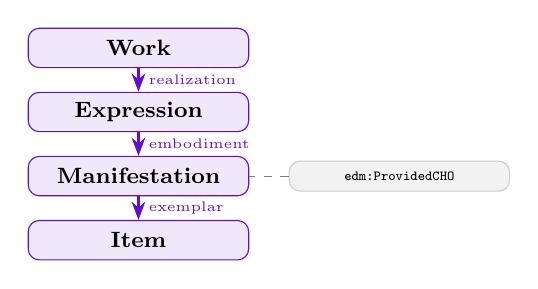
\begin{tikzpicture}[
          wemi/.style={draw=maincolor, fill=maincolor!10, rounded corners,
                       font=\footnotesize\bfseries, minimum width=2.8cm,
                       minimum height=0.5cm, align=center},
          sub/.style={font=\tiny, fill=gray!10, draw=gray!40, rounded corners,
                      minimum width=2.8cm, minimum height=0.38cm, align=center},
          arr/.style={-Stealth, maincolor, thick}
        ]
          \node[wemi] (W) {Work};
          \node[wemi] (E) [below=0.3cm of W]  {Expression};
          \node[wemi] (M) [below=0.3cm of E]  {Manifestation};
          \node[wemi] (I) [below=0.3cm of M]  {Item};
          \node[sub]  (edm) [right=0.5cm of M] {\texttt{edm:ProvidedCHO}};
          \draw[arr] (W) -- (E) node[midway,right,font=\tiny]{realization};
          \draw[arr] (E) -- (M) node[midway,right,font=\tiny]{embodiment};
          \draw[arr] (M) -- (I) node[midway,right,font=\tiny]{exemplar};
          \draw[dashed, gray] (edm) -- (M);
        \end{tikzpicture}
      \end{block}
      \smallskip
      \footnotesize
      Pattern 1 example:
      \begin{center}
        \texttt{<ddb/12345> a edm:ProvidedCHO,}\\
        \texttt{\hspace{1.2cm} mocho:Manifestation ;}\\
        \texttt{\hspace{1.2cm} mocho:realizationOf <gnd:Faust> .}
      \end{center}
    \end{column}
  \end{columns}
\end{frame}

% ===== 3. GOETHE/FAUST EXAMPLE =====

\begin{frame}{Running Example: Goethe's \textit{Faust} across Five Domains}
  \small
  \textbf{Five DDB objects --- one Work (\texttt{gnd:4018116-6}), five sectors:}
  \medskip
  \begin{center}
  \begin{tabular}{llll}
    \toprule
    Object & Sector & WEMI & EDM alone \\
    \midrule
    Book edition (1826)            & Library    & Manifestation & isolated \texttt{ProvidedCHO} \\
    Portfolio of hand illustrations & Museum     & Item          & isolated \texttt{ProvidedCHO} \\
    1893 Weimar playbill            & Archive    & Item          & isolated \texttt{ProvidedCHO} \\
    1926 film still (C.\ Horn)     & Media Lib. & Item          & isolated \texttt{ProvidedCHO} \\
    Jewel song recording (Gounod)  & Media Lib. & Expression    & isolated \texttt{ProvidedCHO} \\
    \bottomrule
  \end{tabular}
  \end{center}
  \medskip
  \begin{columns}
    \begin{column}{.48\textwidth}
      \begin{block}{Without MOCHO}
        Five dead-end records.
        ``Find all Manifestations of \textit{Faust}'' requires knowing all five
        providers, five schemas, five uncontrolled \texttt{dc:type} strings.
      \end{block}
    \end{column}
    \begin{column}{.48\textwidth}
      \begin{exampleblock}{With MOCHO}
        One SPARQL query over \texttt{mocho:Work <gnd:Faust>} returns all five,
        with typed roles, agent relationships, and cross-sector faceting.
      \end{exampleblock}
    \end{column}
  \end{columns}
\end{frame}

% ===== 4. GeMeA SYSTEM =====
\section{GeMeA}

\begin{frame}{GeMeA: German Memory Atlas}
  \begin{columns}
    \begin{column}{.52\textwidth}
      \textbf{Knowledge graph browser for the DDB.}
      \medskip
      \begin{itemize}\setlength{\itemsep}{4pt}
        \item \textbf{27M+ objects} ingested from all 7 DDB sectors
        \item \textbf{QLever} SPARQL triplestore
              (top Sparqloscope benchmarks; built-in text + spatial)
        \item \textbf{SHMARQL} --- lightweight Linked Data publishing layer:
              browsable web UI + \texttt{/sparql} endpoint
        \item \textbf{MCP/MCPO} agentic access layer ---
              novel interface for LLM + KG research
        \item Mocho alignment PoC on representative subset
      \end{itemize}
      \medskip
      \begin{block}{Testbed opportunities}
        \footnotesize
        KG-grounded retrieval (SPARQL-assisted RAG) $\cdot$
        entity-linked QA $\cdot$
        ontology evaluation $\cdot$
        provenance modelling (PROV-O) $\cdot$
        entity embedding benchmarks
      \end{block}
    \end{column}
    \begin{column}{.45\textwidth}
      \begin{center}
      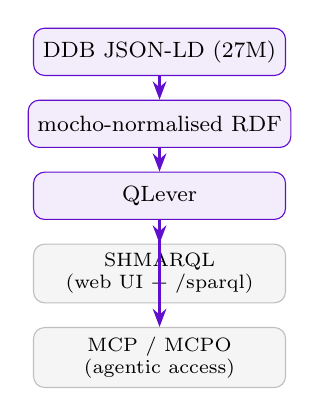
\begin{tikzpicture}[
        box/.style={draw=maincolor, fill=maincolor!8, rounded corners,
                    font=\footnotesize, align=center,
                    minimum width=3.2cm, minimum height=0.6cm},
        sbox/.style={draw=gray!50, fill=gray!8, rounded corners,
                     font=\scriptsize, align=center,
                     minimum width=3.2cm, minimum height=0.5cm},
        arr/.style={-Stealth, maincolor, thick}
      ]
        \node[box] (qlever)  {QLever};
        \node[sbox] (sh) [below=0.3cm of qlever] {SHMARQL\\(web UI + /sparql)};
        \node[sbox] (mcp)[below=0.3cm of sh]      {MCP / MCPO\\(agentic access)};
        \draw[arr] (qlever) -- (sh);
        \draw[arr] (qlever) -- (mcp);
        \node[box] (mocho) [above=0.3cm of qlever] {mocho-normalised RDF};
        \draw[arr] (mocho) -- (qlever);
        \node[box] (ddb) [above=0.3cm of mocho] {DDB JSON-LD (27M)};
        \draw[arr] (ddb) -- (mocho);
      \end{tikzpicture}
      \end{center}
      \smallskip
      \footnotesize
      \textbf{Target}: ISWC 2026 Resource Track\\
      Abstract: 2 May $\cdot$ Paper: 7 May 2026
    \end{column}
  \end{columns}
\end{frame}

% ===== 5. PIPELINE =====

\begin{frame}{Ingest Pipeline}
  \small
  \begin{center}
  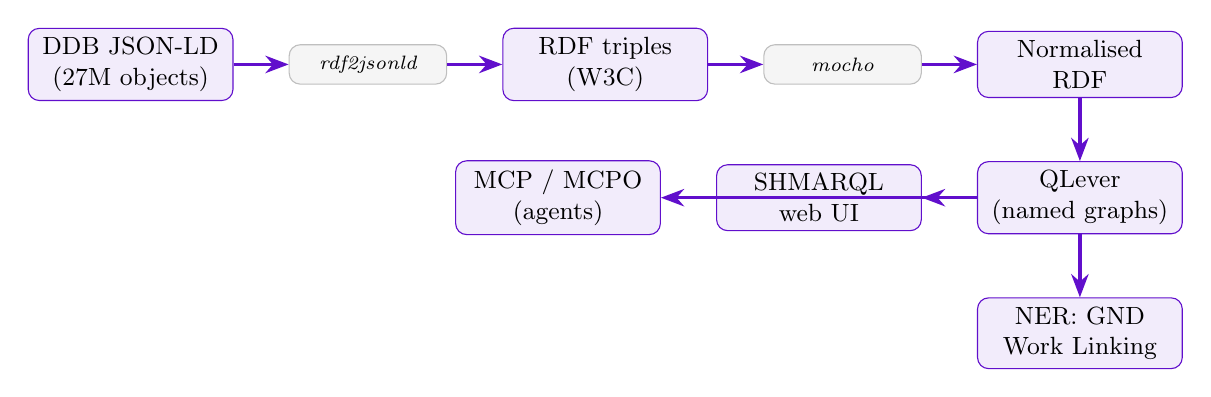
\begin{tikzpicture}[
    stage/.style={draw=maincolor, fill=maincolor!8, rounded corners,
                  font=\small, align=center,
                  minimum width=2.6cm, minimum height=0.65cm},
    tool/.style={draw=gray!50, fill=gray!8, rounded corners,
                 font=\scriptsize\itshape, align=center,
                 minimum width=2.0cm, minimum height=0.5cm},
    arr/.style={-Stealth, maincolor, very thick},
    note/.style={font=\scriptsize\color{gray}, align=left}
  ]
    \node[stage] (ddb)     {DDB JSON-LD\\(27M objects)};
    \node[tool]  (r2j)     [right=0.7cm of ddb]    {rdf2jsonld};
    \node[stage] (rdf)     [right=0.7cm of r2j]    {RDF triples\\(W3C)};
    \node[tool]  (mch)     [right=0.7cm of rdf]    {mocho};
    \node[stage] (norm)    [right=0.7cm of mch]    {Normalised\\RDF};
    \node[stage] (qlv)     [below=0.8cm of norm]   {QLever\\(named graphs)};
    \node[stage] (shmq)    [left=0.7cm  of qlv]    {SHMARQL\\web UI};
    \node[stage] (mcp2)    [left=0.7cm  of shmq]   {MCP / MCPO\\(agents)};
    \node[stage] (ner)     [below=0.8cm of qlv]    {NER: GND\\Work Linking};

    \draw[arr] (ddb)  -- (r2j);
    \draw[arr] (r2j)  -- (rdf);
    \draw[arr] (rdf)  -- (mch);
    \draw[arr] (mch)  -- (norm);
    \draw[arr] (norm) -- (qlv);
    \draw[arr] (qlv)  -- (shmq);
    \draw[arr] (qlv)  -- (mcp2);
    \draw[arr] (qlv)  -- (ner);
  \end{tikzpicture}
  \end{center}

  \begin{columns}
    \begin{column}{.32\textwidth}
      \begin{block}{Scale}
        \footnotesize
        27M objects $\cdot$ 7 sectors $\cdot$
        $\sim$650M triples (est.)
      \end{block}
    \end{column}
    \begin{column}{.32\textwidth}
      \begin{block}{Open access}
        \footnotesize
        Public SPARQL endpoint $\cdot$
        CC BY 4.0 $\cdot$ Stable W3ID URIs
      \end{block}
    \end{column}
    \begin{column}{.32\textwidth}
      \begin{block}{Status (v1)}
        \footnotesize
        115K Goethe--Faust pilot $\checkmark$\\
        Full corpus ingest: in progress
      \end{block}
    \end{column}
  \end{columns}
\end{frame}

% ===== 6. NER CHALLENGE =====
\section{NER}

\begin{frame}{GND Work Linking: The NER Challenge}
  \begin{columns}
    \begin{column}{.52\textwidth}
      \textbf{Goal:} link DDB Manifestation records to GND Works
      via extracted title fields.
      \medskip

      \textbf{Corpus:} 9.21M German-language DDB records
      (Library sector; \texttt{dc:language} $\in$ \{ger, gmh, nds, lat\};
      ADR-01 htype filter).
      \medskip

      \begin{block}{Why NER?}
        \textbf{92.4\% (8.5M records)} are tier-0 ---
        ISBD signals present but insufficient for
        reliable automatic labeling.\\
        $\Rightarrow$ NER is the primary extraction path.
      \end{block}
      \medskip

      \textbf{Labels (Phase 1):}
      \begin{itemize}\setlength{\itemsep}{2pt}
        \item \texttt{TITLE} --- title proper
        \item \texttt{OTHER\_TITLE} --- subtitle (after \texttt{ :})
        \item \texttt{PERSON} --- statement of responsibility (after \texttt{ /})
      \end{itemize}
      \smallskip
      \footnotesize
      Minimum set for FRBR Work-level identity
      $\to$ GND \textit{Werk} lookup.
    \end{column}
    \begin{column}{.45\textwidth}
      \textbf{Why off-the-shelf NER fails:}
      \smallskip
      \begin{enumerate}\setlength{\itemsep}{3pt}
        \item \textbf{Wrong labels} --- standard models
              have \texttt{PER/ORG/LOC}, no \texttt{TITLE}
        \item \textbf{Wrong domain} --- ISBD strings are
              structured records, not prose
        \item \textbf{Historical register} ---
              pre-1750: author credentials precede the
              title with no punctuation marker;
              Early Modern German orthography
        \item \textbf{NuNER Zero ruled out} ---
              SR-09 (zero-shot sanity check):
              F1\,=\,0.000 across all labels
      \end{enumerate}
      \smallskip
      \begin{alertblock}{Confirmed path}
        \footnotesize
        LLM annotation + fine-tuned \texttt{xlm-roberta-base}
      \end{alertblock}
    \end{column}
  \end{columns}
\end{frame}

% ===== 7. SILVER DATASET =====

\begin{frame}{Silver Dataset: ISBD-Based Automatic Labeling at Scale}
  \small
  \begin{columns}
    \begin{column}{.48\textwidth}
      ISBD punctuation signals map directly to labels ---
      no human annotation needed for the silver tier:
      \smallskip
      \begin{center}
      \begin{tabular}{lll}
        \toprule
        Signal & Label & Coverage \\
        \midrule
        \texttt{ :}   & \texttt{OTHER\_TITLE} & 37.5\% \\
        \texttt{ /}   & \texttt{PERSON}$^\dagger$ & 0.5\% \\
        4-digit year  & (Manifestation) & 20.0\% \\
        \texttt{. -}  & Area separator  & 0.4\% \\
        \texttt{ =}   & \xmark~80\% FP  & excluded \\
        Trailing .    & \xmark~93\% FP  & excluded \\
        \bottomrule
      \end{tabular}
      \end{center}
      \footnotesize
      $^\dagger$ \texttt{ /} requires sub-classification:
      36\% FP as PERSON; 41\% non-SoR false positives.
    \end{column}
    \begin{column}{.48\textwidth}
      \textbf{Three silver tiers:}
      \smallskip
      \begin{tabular}{llrr}
        \toprule
        Tier & Criterion & Share & Count \\
        \midrule
        \textbf{2} Structural  & \texttt{has\_dot\_dash} + multi-field & 0.1\% & 7,105 \\
        \textbf{1} Heuristic   & $\geq$3 signals, or person+year & 7.5\% & 689K \\
        \textbf{0} Fallback    & no convergent signal & \textbf{92.4\%} & 8.52M \\
        \bottomrule
      \end{tabular}
      \medskip

      \begin{block}{Key result}
        \footnotesize
        Tier percentages \textbf{stable} across both corpora (pkl 4.47M
        and parquet 9.21M) --- ISBD heuristics scale uniformly.
        Pre-1700: only \textbf{7 tier-2 records} ---
        pre-ISBD conventions predate area separators.
      \end{block}
    \end{column}
  \end{columns}
\end{frame}

% ===== 8. EVALUATION =====

\begin{frame}{Evaluation Framework}
  \small
  \begin{columns}
    \begin{column}{.52\textwidth}
      \textbf{Strata defined by NER difficulty,} not corpus size.
      Primary signal: median BPE token length per era.
      \medskip

      \footnotesize
      \begin{tabular}{lrrl}
        \toprule
        Era & Corpus & Med.\ words & Key challenge \\
        \midrule
        Pre-1700   & 403K  & \textbf{18} & Author-before-title; no ISBD \\
        1700--1800 & 654K  & 10          & ISBD adoption $\sim$1750; mixed \\
        19th-c     & 3.74M &  6          & Serials; corporate SoRs \\
        Modern     & 3.83M &  8          & Subtitles in separate field \\
        \bottomrule
      \end{tabular}
      \smallskip\small

      Gold: 130 / 80 / 60 / 80 = 350 records (+45 dc\_type draw = 395 total).\\
      Oversampled: Leichenpredigt \& Einblattdruck ($\sim$40--50 each).
    \end{column}
    \begin{column}{.45\textwidth}
      \textbf{Metric:} exact span match per label per era.
      \smallskip
      \begin{tabular}{lll}
        \toprule
        Stratum & TITLE & PERSON \\
        \midrule
        Modern   & $\geq$0.85 & --- \\
        19th-c   & $\geq$0.80 & --- \\
        1700--1800 & $\geq$0.75 & $\geq$0.70 \\
        Pre-1700   & $\geq$0.70 & $\geq$0.70 \\
        \bottomrule
      \end{tabular}
      \smallskip

      \begin{block}{CI constraints}
        \footnotesize
        $\pm$10\,pp (Wilson) on TITLE; PERSON CI not
        achievable at practical cost (0.2--8.7\%
        prevalence). Wide CI on PERSON acknowledged
        explicitly; reported as indicative.
      \end{block}

      \begin{alertblock}{Benchmarks (ceiling)}
        \footnotesize
        HIPE-2022 sonar (19C German): best F1\,=\,0.529\\
        OntoNotes WORK\_OF\_ART: 0.532
      \end{alertblock}
    \end{column}
  \end{columns}
\end{frame}

% ===== 9. SUMMARY + COLLABORATION =====
\section{Summary}

\begin{frame}{Summary and Collaboration Opportunities}
  \begin{columns}
    \begin{column}{.57\textwidth}
      \textbf{Three connected contributions:}
      \begin{enumerate}\setlength{\itemsep}{4pt}
        \item \textbf{babel-ddb / MOCHO} --- mid-level ontology for
              cross-domain CH alignment; four alignment patterns;
              applicable to Europeana, DPLA, Gallica
        \item \textbf{GeMeA} --- first openly SPARQL- and
              MCP-accessible KG over the DDB (27M objects);
              testbed for LLM + KG research at CH scale
        \item \textbf{NER pipeline} --- silver + gold datasets for
              bibliographic title string segmentation;
              fine-tuned XLM-R for GND Work linking
      \end{enumerate}
      \medskip
      \textbf{Open questions for collaboration:}
      \begin{itemize}\setlength{\itemsep}{2pt}
        \item MOCHO formalisation, publication, user study
        \item LLM annotation pipeline; cross-lingual NER
        \item LLM + KG benchmarks on GeMeA (RAG, QA, agents)
        \item Provenance modelling of LLM-assisted KG enrichment
        \item Extension to Europeana, DPLA, national aggregators
      \end{itemize}
    \end{column}
    \begin{column}{.40\textwidth}
      \begin{center}
        \uncover<2->{
          \textbf{Thank you for your attention!}\\[0.4cm]
          \Huge \textcolor{maincolor}{\Smiley}\\[0.5cm]
          \normalsize
          \textbf{Mary Ann Tan}\\
          FIZ Karlsruhe, KDAI\\[0.2cm]
          \footnotesize
          \textcolor{maincolor}{mary-ann.tan@fiz-karlsruhe.de}
        }
      \end{center}
    \end{column}
  \end{columns}
\end{frame}

\end{document}
